\emph{This page is for people who want to help develop/improve this
handbook.}

\emph{If you want to get involved,~write to
\href{http://en.wikipedia.org/wiki/Howard\_Rheingold}{Howard Rheingold}
at~\href{mailto:howard@rheingold.com}{howard@rheingold.com}.}

\emph{Illustrations by \href{http://www.visualsforchange.com/}{Amanda
Lyons}.}

\begin{center}
\href{http://peeragogy.org/wp-content/uploads/2012/03/welcome\_color.gif}{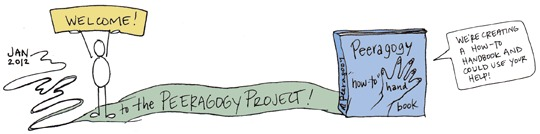
\includegraphics[width=.9\textwidth]{./pictures/welcome_color.jpg}}
\end{center}

\subsection{Hello and welcome!}

The peeragogy project was kicked off around the time of
\href{http://rheingold.com/}{Howard Rheingold's} January 23,
2012~\href{http://vimeo.com/35685124}{Regents Lecture} at UC Berkeley.~
We now have a complete first draft of a handbook e-book for peer
learning (the website you're reading!). There's still more work to be
done --- and this page assumes you're interested in getting involved.~
In that case: we're happy to have you aboard, and what you do here is
largely up to you. Go through the orientation material on our
\href{http://socialmediaclassroom.com/host/peeragogy}{Wiki}. Poke
around. Ask questions --- we're eager to answer them. Find an area where
you feel knowledgeable (or are willing to learn) and have a passion to
contribute.

\begin{center}
\href{http://peeragogy.org/wp-content/uploads/2012/03/what\_to\_do\_color.gif}{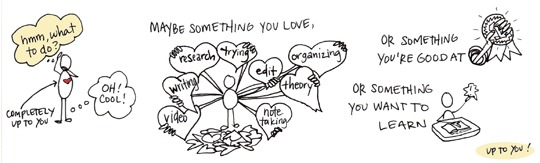
\includegraphics[width=.9\textwidth]{./pictures/what_to_do_color.jpg}}
\end{center}

The goal of this e-book is to be a USEFUL guide to peer learning (have a
look at
\href{http://socialmediaclassroom.com/host/peeragogy/wiki/initial-outline-source-book}{the
outline})! To achieve that goal we have multiple opportunities for peers
to contribute:

\begin{itemize}
\item
  add relevant links to pages.
\item
  write the text for a sub-section (like this one you're currently
  reading),
\item
  organize a team to tackle a larger section,
\item
  make a video (like these on our
  \href{http://www.youtube.com/channel/UCIQY4ja8e4Br-i9U5KnmyZQ}{YouTube
  Channel}),
\item
  take notes of live meetings or
  \href{http://cmapspublic3.ihmc.us/rid=1K81VLSK7-1RL0RQ4-WZK/Peeragogy\%20Cmap.cmap}{grow
  concept maps,}
\item
  organize a newsletter for your group or the whole team,
\item
  add general purpose bookmarks to
  \href{http://groups.diigo.com/group/peeragogy-handbook}{this Diigo
  group}, or post comments and editorial notes about peeragogy.org in
  \href{http://groups.diigo.com/group/peering-into-peeragogy\%20}{this
  one}; and
\item
  discuss peer learning matters and this handbook informally via our
  forums.
\end{itemize}

It's up to you. We do have norms and standards that've emerged from
back-and-forth discussion and resist ready codification. Instead of
reading a list of rules, join our conversations, take advantage of the
digital memory of a forum to rewind the conversation back closer to the
beginning, figure out what the community is like, and jump in. We won't
know you've jumped in, though, until you communicate with us about what
you'd like to do, who and how you'd like to help, how you think we ought
to do it. You can have a look at the outstanding tasks and teams that
are listed on
\href{https://docs.google.com/document/d/1\_2I-z-Pt5NUKk-fpy4jsqxFeXbWS4ao4sIhkxCcRVeI/edit\#}{this
Google Doc}.

\begin{center}
\href{http://peeragogy.org/wp-content/uploads/2012/03/lots\_going\_on\_color\_1000.gif}{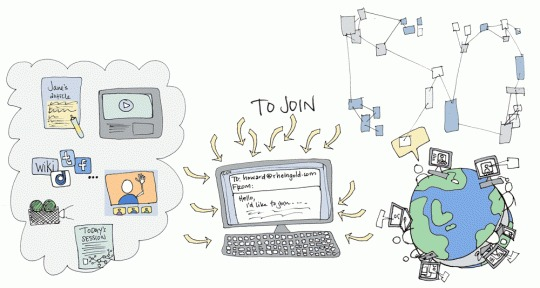
\includegraphics[width=.9\textwidth]{./pictures/lots_going_on.jpg}}
\end{center}

\subsection{Where to go, what to do when you get there, to learn about
how we work}

We use the forums to communicate asynchronously and continuously. We
also meet irregularly for synchronous audio-video sessions. Information
and answers about both methods of communication can be found in the
forums.

\begin{center}
\href{http://peeragogy.org/wp-content/uploads/2012/03/where\_to\_go\_color.gif}{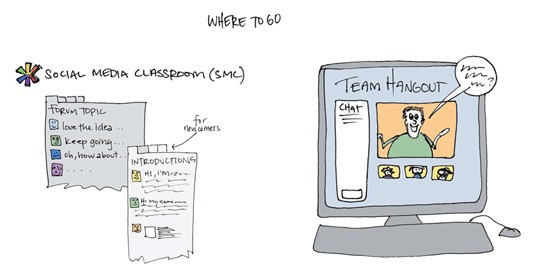
\includegraphics[width=.9\textwidth]{./pictures/where_to_go_color.jpg}}
\end{center}

Click on \href{http://socialmediaclassroom.com/host/peeragogy/forum}{the
forums tab}. Each forum is a container for conversation threads that can
continue for months. The How-to tab can show you how to navigate the
forums. Please
\href{http://socialmediaclassroom.com/host/peeragogy/forum/please-introduce-yourself}{introduce
yourself}! After that, the first place you'll want to go is
the~\href{http://socialmediaclassroom.com/host/peeragogy/forum/newcomers-start-here-welcome-center}{newcomer
forum topic}, where you can get useful information and ask questions
about how things work around here, how to get started. In
\href{http://socialmediaclassroom.com/host/peeragogy/forum/recaps-and-updates-forum-wiki-tools-handbook-activity}{this
thread} you'll find a weekly recap of activity in the forums, wiki, live
meetings.

\subsection{Workflow: How to Create Content for the Handbook}

\begin{enumerate}
\item
  Sign up for a project team in the forum or create one by proposing it
  in a new comment thread in
  the~\href{http://socialmediaclassroom.com/host/peeragogy/forums/project-teams}{Project
  Teams forum}.
\item
  Communicate with other team members through whatever media works best
  for you -- forum, wiki comments, G+Hangouts, Skype, face to face. Do
  share what you discuss/decide in the forum.
\item
  Create content on
  the~\href{http://socialmediaclassroom.com/host/peeragogy/wiki/main-page}{Handbook
  wiki}, or in any place you'd like that is linked
  from~\href{http://socialmediaclassroom.com/host/peeragogy/wiki/initial-outline-source-book}{the
  wiki outline}.
\item
  ~\href{http://socialmediaclassroom.com/host/peeragogy/forum/editorial-team}{Tell
  the editorial team}~that you are ready for an editorial once-over.
  Make sure you've signed
  the~\href{http://socialmediaclassroom.com/host/peeragogy/wiki/license}{CC0
  Copyright Waiver}~(``License'') so that we have permission to
  redistribute your work without restrictions.
\item
  Editorial team looks at material, communicates with original content
  creators if necessary, edits content.
\item
  Editorial team and content creation team sign off on the content.~
  When the content is ready to be moved over it will be labled ``RFWP''
  next to the content on
  \href{http://socialmediaclassroom.com/host/peeragogy/wiki/initial-outline-source-book}{the
  wiki outline}.
\item
  The WordPress Team is creating the Table of Contents, and Menu for the
  site.~ When your content is ready, we will create empty posts for you
  to copy over your content into on the Wordpress site, and add them to
  the table of contents.
\item
  One member of your Project Team (or more if needed) should volunteer
  themselves to move over your content.~ The WordPress Team will create
  a username and login for that WP Project Team Editor.~ If you are a WP
  Editor for your Team,~ please post to let us know in the
  \href{http://socialmediaclassroom.com/host/peeragogy/forum/the-wordpress-site}{WordPress
  Site Forum} and we will add you as an editor.~ We will need your email
  address in order to email you your password.
\item
  Once the content has been moved over, mark it in the wiki outline as
  ``moved to WP'' and content should then be edited there.~ Make sure to
  mark your article in the wiki as ``moved to wordpress - view/edit here
  \textless{}insert your link\textgreater{}''.
\item
  Formatting your post:~ We will (this is not done yet) use these sample
  posts for formatting consistency:
  ~\href{http://peeragogy.org/how-to-get-involved/}{How to Get
  Involved}~page and the
  \href{http://peeragogy.org/connectivism-in-practice-how-to-organize-a-mooc/}{How
  to Organize a MOOC} page.~You will be able to use these as examples of
  how to format your post.
\end{enumerate}

\subsection{How to join or start your own project team}

\begin{itemize}
\item
  \href{http://socialmediaclassroom.com/host/peeragogy/forum/teaming-signing-flesh-out-parts-outline}{The
  forum thread about volunteering to help create the handbook.}~It's not
  a contract, but it's a public commitment to say ``I'll do that'' or
  ``I can help with that.''
\item
  \href{http://socialmediaclassroom.com/host/peeragogy/forum/initial-rough-outline}{This
  is where we talk about what ought to go in the handbook}, how to
  organize the outline.
\item
  The~\href{http://socialmediaclassroom.com/host/peeragogy/forums/project-teams}{Project
  Teams forum}~-- Take a look at the Project Teams and jump in wherever
  you find a task that interests you.
\end{itemize}

\href{http://peeragogy.org/wp-content/uploads/2012/03/create\_content.gif}{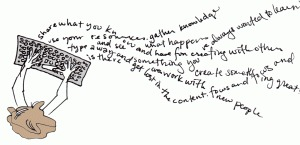
\includegraphics{./pictures/create_content.jpg}}

\subsection{Details About the Wiki}

\begin{itemize}
\item
  WIKI BASICS -~Get a look at what people have created using this
  \href{http://socialmediaclassroom.com/host/peeragogy/wikichanges}{Recent
  Changes}page.

  \begin{itemize}
  \item
    CREATING A PAGE -~To create a new wiki page, linked from an existing
    page: Edit the existing wiki page, type or choosen anchor text to
    link to your new page, enclose the anchor text in in double
    brackets, submit the page, click on the new link, create a wiki
    page, edit its contents, submit. This process is described
    under\href{http://socialmediaclassroom.com/host/peeragogy/page/how}{~the
    How-to tab}~as
    "\href{http://socialmediaclassroom.com/host/peeragogy/slideshow/creating-a-new-wiki-page}{Creating
    a New Wiki Page}".
  \item
    TEMPLATE FOR ENTRIES -~Make sure that this is a
    how-to-do-it-oriented resources. Scaffold with just enough theory,
    explained without special jargon, to make the how-to-do-it clear.
    Link to the literature review (and add to the lit review if
    necessary) for more detailed discussion of empirical, scholarly,
    theoretical underpinnings of the how-to-do-it. Each page should
    have:

    \begin{itemize}
    \item
      \textbf{Set of tags}: Specify a set of tags you would like used to
      refer to material related to this entry.
    \item
      \textbf{A ``Status'' line at the very top}, indicating whether it
      is a stub, an outline for a completed article, a draft in
      progress, a draft ready for editing, or a draft edited and ready
      to move to Wordpress.
    \item
      \textbf{A list of content creators and editors}~after the Status
      line.
    \item
      \textbf{Short summary under the creators/editors list~}: Start and
      maintain a summary (under approximately 300 words) above the body
      of your entry, either a category or sub-category.
    \item
      \textbf{Source citations and Resources:}~Make sure direct
      quotations of material that are not the content creators' own
      words are clearly identified with quotation marks, immediately
      followed with enough information for readers to find bibliographic
      information and/or URLs for all cites in the Resources section;
      cited sources should be listed with all bibliographic information
      and URL in ~the overall list of resources. When you have drafted
      or substantially changed an entry, the owner should notify the
      owner of the Resources entry.
    \item
      \textbf{Links to related pages.}~If another part of the Handbook
      is particularly relevant, link to it.
    \item
      \textbf{Link back to main page of the outline}: Each page should
      include at the bottom a large link back to the main page of the
      outline.
    \item
      A good example of a page that has all these elements, well
      composed,
      is~\href{http://socialmediaclassroom.com/host/peeragogy/wiki/connectivism-practice-how-organize-a-mooc}{Connectivism
      in Action: How to Organize a MOOC}.
    \item
      COMMENT THREADS ATTACHED TO WIKI PAGES -~Adding a comment to a
      wiki page will start a comment thread or append the new comment to
      the existing thread in chronological order. Comment threads on
      wiki pages can focus on discussions of the specific additions and
      changes proposed to this wiki team by the project team members for
      this entry. You can toggle between a wiki page and a page of
      comments by means of the ``Talk'' tab, next to the View, Edit,
      Outline, Revisions, and Access control tabs.
    \end{itemize}
  \end{itemize}
\end{itemize}

\textbf{\href{http://peeragogy.org/wp-content/uploads/2012/03/communicate\_color1.gif}{
\includegraphics{./pictures/communicate.jpg}}}

\subsection{How we Communicate}

FORUMS -~The asynchronous (participate whenever you'd like)
conversations in the forums are how the community of peeragogy handbook
creators formed. It's where we engage in exended discussions of issues
and decisions raised in live sessions. It's where we keep track of which
different teams are working on which material. It's where the small
teams can engage with the community as a whole. It's a place to ask
questions, propose changes, volunteer to help, hand off work to the next
team.

LIVE SESSIONS -~We meet synchronously at agreed-upon times, using audio,
video, text chat, slides, screen-sharing. For groups of ten or more, we
use Blackboard Collaborate, for which Howard has a 50-seat-at-a-time
license. These sessions are recorded. For information about scheduling,
and recordings,
see~\href{http://socialmediaclassroom.com/host/peeragogy/forum/live-sessions-schedule-recordings-notes-mindmaps}{the
forum topic}. Participation requires a fairly fast (broadband) Internet
connection, a microphone or headset, and (if you wish), a webcam. For
groups of ten or smaller (usually for project teams), we use Google+
Hangouts. Individual teams do their own scheduling.

TWITTER LIST - Follow \href{http://twitter.com/Peeragogy/}{@Peeragogy}
\& to get added to the Peeragogy Twitter list please post your Twitter
name
\href{http://socialmediaclassroom.com/host/peeragogy/forum/the-tools-we-are-using-and-how-access-them}{here}.
Stephanie Schipper will then add you.

TWITTER HASHTAG:
\href{http://twitter.com/search?q=\%23peeragogy\&src=typd}{\#peeragogy}
\href{https://www.facebook.com/peeragogy}{FACEBOOK PAGE} \textbf{~
\href{http://peeragogy.org/wp-content/uploads/2012/03/questions\_1000.gif}{
\includegraphics{./pictures/questions.jpg}}}

\subsection{Questions?}

If you have questions, use the forums, post a comment on the Talk page
for this wiki entry, email the team energy center, or
email~\href{mailto:howard@rheingold.com}{howard@rheingold.com}
